\documentclass[border=5pt]{standalone}
\usepackage{tikz}
\usepackage{amsmath}
\usepackage{amssymb}
\usepackage{helvet}
\usepackage{pifont}
\renewcommand{\familydefault}{\sfdefault}
\usetikzlibrary{shapes.geometric, arrows.meta, positioning, fit, backgrounds, decorations.pathreplacing, shadows}

\newcommand{\cmark}{\ding{51}}   % ✓
\newcommand{\xmark}{\ding{55}}   % ✗
\newcommand{\warnmark}{(!)}      % ⚠ substitute


% ── colour palette ──────────────────────────────────────────────
\definecolor{blk1bg}{RGB}{219,234,254}   % sky-blue fill  (block 1)
\definecolor{blk1bd}{RGB}{ 37,99,235}    % blue border
\definecolor{blk2bg}{RGB}{220,252,231}   % green fill     (block 2)
\definecolor{blk2bd}{RGB}{ 22,163, 74}   % green border
\definecolor{blk3bg}{RGB}{255,237,213}   % orange fill    (block 3)
\definecolor{blk3bd}{RGB}{234, 88,  12}  % orange border
\definecolor{blk4bg}{RGB}{243,232,255}   % purple fill    (block 4)
\definecolor{blk4bd}{RGB}{147, 51,234}   % purple border
\definecolor{arrowcol}{RGB}{ 55, 65, 81} % dark-gray arrows
\definecolor{attackred}{RGB}{220, 38, 38}
\definecolor{headerbg}{RGB}{ 15, 23, 42} % near-black header

\tikzset{
  blkbase/.style={
    rectangle, rounded corners=4pt, minimum width=3.6cm,
    text width=3.5cm, align=left, inner sep=6pt,
    drop shadow={shadow xshift=1pt, shadow yshift=-1pt, opacity=0.15}
  },
  hdr/.style={
    rectangle, rounded corners=3pt, minimum width=3.6cm,
    text width=3.5cm, align=center, inner sep=4pt,
    font=\bfseries\footnotesize\color{white}, fill=headerbg
  },
  blk1/.style={blkbase, fill=blk1bg, draw=blk1bd, line width=1pt},
  blk2/.style={blkbase, fill=blk2bg, draw=blk2bd, line width=1pt},
  blk3/.style={blkbase, fill=blk3bg, draw=blk3bd, line width=1pt},
  blk4/.style={blkbase, fill=blk4bg, draw=blk4bd, line width=1pt},
  myarrow/.style={-{Latex[length=3mm,width=2mm]}, line width=1.5pt, color=arrowcol},
  healback/.style={{Latex[length=3mm,width=2mm]}-, line width=1.5pt, color=attackred, dashed},
  buslabel/.style={circle, draw, fill=white, inner sep=1pt, font=\tiny, minimum size=11pt},
  attackbus/.style={circle, draw=attackred, fill=red!15, inner sep=1pt, font=\tiny\bfseries\color{attackred}, minimum size=11pt},
}

\begin{document}
\begin{tikzpicture}[node distance=0.55cm]

% ═══════════════════════════════════════════════════════════
%  BLOCK 1 — Physical Smart Grid
% ═══════════════════════════════════════════════════════════
\node[hdr, fill=blk1bd] (h1) {Physical Smart Grid\\[-1pt]SCADA Layer};

\node[blk1, below=0pt of h1] (b1) {%
  % ── mini 14-bus topology ──
  \begin{tikzpicture}[scale=0.62, every node/.style={font=\tiny}]
    % nodes
    \node[buslabel] (n1)  at (0.0,1.6)  {1};
    \node[buslabel] (n2)  at (1.1,2.2)  {2};
    \node[buslabel] (n3)  at (2.2,2.4)  {3};
    \node[buslabel] (n4)  at (3.0,1.8)  {4};
    \node[attackbus](n5)  at (2.8,0.8)  {5};
    \node[buslabel] (n6)  at (1.8,0.2)  {6};
    \node[buslabel] (n7)  at (1.0,0.8)  {7};
    \node[buslabel] (n8)  at (0.1,0.4)  {8};
    \node[buslabel] (n9)  at (3.6,2.4)  {9};
    \node[buslabel] (n10) at (4.2,1.6)  {10};
    \node[buslabel] (n11) at (3.8,0.8)  {11};
    \node[buslabel] (n12) at (3.0,0.1)  {12};
    \node[buslabel] (n13) at (2.0,1.3)  {13};
    \node[buslabel] (n14) at (4.4,0.2)  {14};
    % edges
    \foreach \a/\b in {n1/n2,n2/n3,n3/n4,n4/n5,n5/n6,n6/n7,n7/n8,n8/n1,
                       n3/n9,n9/n10,n10/n11,n11/n12,n12/n14,n14/n11,
                       n4/n9,n5/n13,n13/n7,n10/n14,n12/n13}{
      \draw[gray!60, line width=0.6pt] (\a)--(\b);
    }
    % attack marker
    \node[font=\tiny\bfseries\color{attackred}] at (2.8, 0.28) {FDIA};
    \draw[-{Latex[length=1.5mm]}, attackred, dashed, line width=0.8pt]
      (4.3,1.1) node[right, font=\tiny, color=attackred] {Adv.} -- (n5);
  \end{tikzpicture}\\[2pt]
  {\scriptsize\color{gray!70!black}
    \textbf{Attack:} $a=h(x{+}c)-h(x)$\\
    \textbf{Stream:} $[V,\theta,P,Q]$\\
    \textbf{BDD:} $\chi^2$ bypassed {\color{attackred}\textbf{\xmark}}
  }
};

% fit header + body
\begin{scope}[on background layer]
  \node[rectangle, rounded corners=5pt, draw=blk1bd, line width=1.5pt,
        fit=(h1)(b1), inner sep=0pt] (box1) {};
\end{scope}

% ═══════════════════════════════════════════════════════════
%  BLOCK 2 — Virtual Graph Twin
% ═══════════════════════════════════════════════════════════
\node[hdr, fill=blk2bd, right=1.1cm of h1] (h2) {Virtual Graph Twin\\[-1pt]$G=(V,E,X,E_{\mathrm{attr}})$};

\node[blk2, below=0pt of h2] (b2) {%
  {\scriptsize
    $x_i=[V_i,\theta_i,P_i,Q_i]^T$\quad (nodes)\\
    $e_{ij}=[R_{ij},X_{ij}]^T$\quad (edges)\\[4pt]
  }
  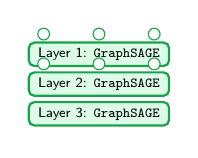
\begin{tikzpicture}[scale=0.54]
    % three GNN layer bars
    \foreach \y/\lbl/\col in {1.5/Layer~1/blk2bd, 0.8/Layer~2/blk2bd, 0.1/Layer~3/blk2bd}{
      \draw[fill=blk2bg, draw=\col, line width=0.8pt, rounded corners=2pt]
        (0,\y) rectangle (3.3,\y+0.55);
      \node[font=\tiny] at (1.65,\y+0.27) {\lbl: \texttt{GraphSAGE}};
    }
    % small node icons in each layer
    \foreach \x in {0.35, 1.65, 2.95}{
      \node[circle, draw=blk2bd, fill=white, inner sep=1.5pt, font=\tiny] at (\x,2.25) {};
      \node[circle, draw=blk2bd, fill=white, inner sep=1.5pt, font=\tiny] at (\x,1.55) {};
    }
  \end{tikzpicture}\\[3pt]
  {\scriptsize\color{gray!70!black}
    $h_v^{(k)}=\mathrm{ReLU}\!\left(W_k\!\left[h_v^{(k-1)}\!\parallel\! h_{\mathcal{N}(v)}^{(k)}\right]\right)$\\[2pt]
    $\mathcal{L}=\mathcal{L}_{\mathrm{BCE}}+1.5\,\mathcal{L}_{\mathrm{WCE}}$
  }
};

\begin{scope}[on background layer]
  \node[rectangle, rounded corners=5pt, draw=blk2bd, line width=1.5pt,
        fit=(h2)(b2), inner sep=0pt] (box2) {};
\end{scope}

% ═══════════════════════════════════════════════════════════
%  BLOCK 3 — Detection & XAI
% ═══════════════════════════════════════════════════════════
\node[hdr, fill=blk3bd, right=1.1cm of h2] (h3) {Detection \& XAI\\[-1pt]Attribution};

\node[blk3, below=0pt of h3] (b3) {%
  {\scriptsize\bfseries Detection Head}\\
  {\scriptsize Graph-level: \textbf{Attack YES} {\color{blk2bd}\cmark}\\
  Det.~F1: \textbf{98.25\%} $\pm$ 0.34\%\\[4pt]}
  {\scriptsize\bfseries Localization Head}\\
  {\scriptsize Node-level: \textbf{Bus 5} {\color{attackred}\warnmark}\\
  Loc.~F1: \textbf{97.62\%} $\pm$ 0.84\%\\[5pt]}
  % IG bar chart
  {\scriptsize\textbf{IG Attribution (Bus 5):}}\\[2pt]
  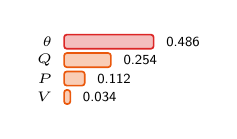
\begin{tikzpicture}[scale=0.9]
    \foreach \val/\lbl/\col/\y in {
      0.486/$\theta$/attackred/0.78,
      0.254/$Q$/blk3bd/0.52,
      0.112/$P$/blk3bd/0.26,
      0.034/$V$/blk3bd/0.0}{
      \draw[fill=\col!30, draw=\col, line width=0.6pt, rounded corners=1pt]
        (0.35,\y) rectangle ({0.35+2.6*\val},\y+0.2);
      \node[font=\tiny, anchor=east] at (0.32,\y+0.1) {\lbl};
      \node[font=\tiny, anchor=west] at ({0.35+2.6*\val+0.04},\y+0.1) {\val};
    }
  \end{tikzpicture}\\[-2pt]
  {\tiny $\sum\!\mathrm{Attr}_i = F(x)-F(x_0)$\quad (complete)}
};

\begin{scope}[on background layer]
  \node[rectangle, rounded corners=5pt, draw=blk3bd, line width=1.5pt,
        fit=(h3)(b3), inner sep=0pt] (box3) {};
\end{scope}

% ═══════════════════════════════════════════════════════════
%  BLOCK 4 — Self-Healing
% ═══════════════════════════════════════════════════════════
\node[hdr, fill=blk4bd, right=1.1cm of h3] (h4) {Closed-Loop\\[-1pt]Self-Healing};

\node[blk4, below=0pt of h4] (b4) {%
  {\scriptsize
    \textbf{Step 1 — Quarantine:}\\
    Mute RTU channels @ Bus~5\\[4pt]
    \textbf{Step 2 — Reconstruct:}\\
    $z_{\mathrm{recon}} = z_{\mathrm{nominal}} \pm \delta$\\
    $\delta\!\sim\!\mathcal{U}(\pm2\%)$\\[5pt]
    \textbf{WLS State Estimation:}\\[2pt]
  }
  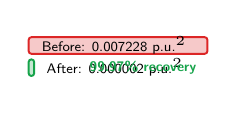
\begin{tikzpicture}[scale=0.88]
    % before/after bar
    \draw[fill=attackred!25, draw=attackred, line width=0.7pt, rounded corners=1pt]
      (0,0.38) rectangle (2.58,0.62);
    \node[font=\tiny, anchor=west] at (0.05,0.50) {Before: 0.007228 p.u.$^2$};
    \draw[fill=blk2bd!25, draw=blk2bd, line width=0.7pt, rounded corners=1pt]
      (0,0.06) rectangle (0.08,0.30);
    \node[font=\tiny, anchor=west] at (0.12,0.18) {After: 0.000002 p.u.$^2$};
    \node[font=\tiny\bfseries\color{blk2bd}] at (1.65,0.18) {99.97\% recovery};
  \end{tikzpicture}\\[3pt]
  {\scriptsize
    Inference loop: \textbf{$<$2 ms}\\
    Latency: \textbf{0.908 ms}\\
    Outage Det.~F1: \textbf{92.80\%}\\
    30-bus Transfer: \textbf{90.11\%}
  }
};

\begin{scope}[on background layer]
  \node[rectangle, rounded corners=5pt, draw=blk4bd, line width=1.5pt,
        fit=(h4)(b4), inner sep=0pt] (box4) {};
\end{scope}

% ═══════════════════════════════════════════════════════════
%  ARROWS between blocks
% ═══════════════════════════════════════════════════════════
\draw[myarrow] (box1.east |- h1) -- node[above, font=\tiny\color{gray!60!black}] {SCADA stream} (box2.west |- h2);
\draw[myarrow] (box2.east |- h2) -- node[above, font=\tiny\color{gray!60!black}] {embeddings} (box3.west |- h3);
\draw[myarrow] (box3.east |- h3) -- node[above, font=\tiny\color{gray!60!black}] {flag Bus 5} (box4.west |- h4);

% Healing feedback arrow (bottom, curved back)
\draw[healback]
  ([yshift=-6pt]box1.south) --
  node[below, font=\tiny\bfseries\color{attackred}] {Quarantine \& Healing Command}
  ([yshift=-6pt]box4.south);

% ═══════════════════════════════════════════════════════════
%  Outer title banner
% ═══════════════════════════════════════════════════════════
\node[above=0.35cm of h2, xshift=2.1cm,
      font=\small\bfseries, text=headerbg] {%
  An Adaptive Explainable Graph Digital Twin for Cyber-Resilient Smart Grids};

\end{tikzpicture}
\end{document}
